\documentclass[12pt]{article}
\usepackage[english]{babel}
\usepackage{natbib}
\usepackage{url}
\usepackage[utf8x]{inputenc}
\usepackage{amsmath}
\usepackage{graphicx}
\usepackage{subfig}
\graphicspath{{../images/}}
\usepackage{parskip}
\usepackage{fancyhdr}
\usepackage{textgreek}
\usepackage{vmargin}
\usepackage{algorithm}
\usepackage[noend]{algpseudocode}
\newcommand{\var}{\texttt}
\usepackage[toc,page]{appendix}

\setmarginsrb{3 cm}{2.5 cm}{3 cm}{2.5 cm}{1 cm}{1.5 cm}{1 cm}{1.5 cm}

\title{Heuristics \& Approximations Algorithms}								% Title
\author{Alexander \& Narongrit}								% Author
\date{27 May 2019}											% Date

\makeatletter
\let\thetitle\@title
\let\theauthor\@author
\let\thedate\@date
\makeatother

\pagestyle{fancy}
\fancyhf{}
\rhead{\theauthor}
\lhead{\thetitle}
\cfoot{\thepage}

\makeatletter
\let\OldStatex\Statex
\renewcommand{\Statex}[1][3]{%
  \setlength\@tempdima{\algorithmicindent}%
  \OldStatex\hskip\dimexpr#1\@tempdima\relax}
\makeatother

\begin{document}

%%%%%%%%%%%%%%%%%%%%%%%%%%%%%%%%%%%%%%%%%%%%%%%%%%%%%%%%%%%%%%%%%%%%%%%%%%%%%%%%%%%%%%%%%

\begin{titlepage}
	\centering
    \vspace*{0.5 cm}
    
\includegraphics[scale = 0.5]{SDU_logo.png}\\[1.0 cm]	% University Logo
    \textsc{\LARGE University of Southern Denmark}\\[2.0 cm]	% University Name
	\textsc{\Large DM852}\\[0.5 cm]				% Course Code
	\rule{\linewidth}{0.2 mm} \\[0.4 cm]
	{ \huge \bfseries \thetitle}\\
	\rule{\linewidth}{0.2 mm} \\[1.5 cm]
	
	\begin{minipage}{0.4\textwidth}
		\begin{flushleft} \large
			\emph{Submitted To:}\\
			Marco Chiarandini\\
            Lene Monrad Favrholdt \\
			IMADA \\
			Mathematics \& Computer Science Department \\
			\end{flushleft}
			\end{minipage}~
			\begin{minipage}{0.4\textwidth}
            
			\begin{flushright} \large
			\emph{Submitted By :} \\
			Alexander Lerche Falk\\
            Narongrit Unwerawattana\\
            Spring - Master of Computer Science\\
		\end{flushright}
        
	\end{minipage}\\[2 cm]
	
	
    
    
    
    
	
\end{titlepage}

%%%%%%%%%%%%%%%%%%%%%%%%%%%%%%%%%%%%%%%%%%%%%%%%%%%%%%%%%%%%%%%%%%%%%%%%%%%%%%%%%%%%%%%%%

\tableofcontents
\pagebreak

%%%%%%%%%%%%%%%%%%%%%%%%%%%%%%%%%%%%%%%%%%%%%%%%%%%%%%%%%%%%%%%%%%%%%%%%%%%%%%%%%%%%%%%%%

\section{Introduction}

This project shows metaheuristic algorithms, resolving the Capacitated Vehicle Routing Problem (CVRP). The difference between metaheuristics and heuristics is in 
the solution part. For heuristics, you are trying your best to find a solution, even though it is not optimal. The algorithm is adapted to the problem
in such a greedy approach, it can get stuck in a local optimum. This is fine since it is the idea of heuristics: "just solve the problem". 
\newline
Metaheuristics are less greedy and tends to be more problem independent. They accept temporary solutions and allow "bad" steps as an attempt to get
a better solution. You have a local- and global optimum to keep track of the best solution found. You can say metaheuristics are exploting
heuristics to avoid getting trapped. 
\newline
In this metaheuristics implementation project, we have chosen to implement two algorithms for CVRP: Simulated Annealing (SA) and Ant Colony Optimization (ACO). 
The SA algorithm is the one we have uploaded for electronic submisison at http://valkyria.imada.sdu.dk/D0App/. The ACO algorithm is implemented but does not perform well.
We will compare the algorithms with our previous heuristic / local search project and lastly, show our results of computation for our two algorithms.

\hspace{1 cm}--- Alexander \& Narongrit

\newpage

\section{Simulated Annealing} 


The Simulated Annealing (SA) algorithm is inspired from the annealing process in metal, where you are altering the physical state of the metal 
by heating and cooling it. The inspiration can be used in computer science as well. We can use the algorithm on CVRP by starting off by generating a solution 
to the problem and not "care" about the initial solutions. The better steps we are taking, and better solutions we are finding, the more careful we are going to be in finding 
a solution. In the beginning we allow random and bad steps to be performed, while later, we make better calculations.
\newline
We have developed an algorithm to solve CVRP using Simulated Annealing technique by relating CVRP with existed problems i.e. 
Bin packing problem and Knapsack problem. Using this approach, we can guarantee maximum amount of vehicles necessary required with approximation analysis on 
bin packing hueristic algorithm. In this demonstration, we use well studied 
algorithm First-Fit-Decreasing which is guaranteed to use no more than $\frac{11}{9}\textsc{OPT} + 1$ number of required vehicles\cite{FFD}. 
With combination of simple Traveling Salesman Problem's local search algorithm, 2-opt, we are able create the initial feasible solution as described 
in~\ref{alg:alg_ffd}. Next step of Simulated Annealing involved creating new feasible solution by altering current solution. 
Which in CVRP case, is to perform points exchange action between routes. In order to allow as much possibility of exchanges as it could without breaking 
capacity constrain, we choose simple algorithm to find exchanges possibility based on Knapsack problem~\ref{alg:alg_knapsackcom}.

\begin{algorithm}[!h]
	\caption{Simulated annealing with First-Fit-Decreasing and Knapsack combination}
	\label{alg:alg_sa}

    \begin{algorithmic}[1]
    \Require{$customers$: List of customer coordinate with it's capacity}

	\Require{$route\_cap(route)$: returns capacity of route} 
	\Require{$route\_cost(route)$: returns capacity of route} 
	\Require{$tsp\_local\_search(route)$: performs travelling salesman local search and returns improved route}
	\Require{$is\_accept(best\_cost, cost, temp)$: an acceptance criterion function returns boolean based on Metopolis condition}

	\Require{$max\_cap$: Maximum capacity for each route} 
	\Require{$depot$: Depot point} 

	\Function{simulated\_annealing\_ffd}{{$customers, temp, alpha, no\_improve\_limits$}}
        \State $routes \gets \textsc{cvrp\_first\_fit\_decreasing}(customers,depot)$
        \State $best\_cost \gets$ total cost of $routes$
        \State $best\_routes \gets routes$
        \State $current\_cost \gets best\_cost$
        \State $current\_routes \gets routes$
        \State $curr\_no\_improve\_trying \gets 0$
        \While{True}
            \If{$curr\_no\_improve\_trying == no\_improve\_limits$}
            break
            \EndIf
            \State $origin\_route\_id, target\_route\_id \gets$ randomly pick 2 distinct index of $routes$
            \State $origin\_route\_point \gets$ randomly pick element from $route[origin\_route\_id]$
            
            \State $upper\_bound, lower\_bound \gets$ maximum and minimum capacity such that solution still feasible after exchange action

            % \State $upper\_bound \gets max\_cap - (route\_cap(routes[origin\_route\_id] - origin\_route\_point.capacity))$

            % \State $lower\_bound \gets route\_cap(routes[target\_route\_id]) - (max\_cap - origin\_route\_point.capacity)$

            \State $target\_neighbors\_set \gets \textsc{knapsack\_combination}($
            \Statex $route[target\_route\_id], lower\_bound, upper\_bound)$

            \If{$len(target\_neighbors\_set) == 0$}
                continue
            \EndIf

            \State $target\_neighbors \gets$ randomly pick an element from $target\_neighbors\_set$

            \State $new\_route\_i, new\_route\_i \gets$ exchange neighbors between two route and assign to new variables

            \State $new\_route\_i \gets tsp\_local\_search(new\_route\_i)$  
            \State $new\_route\_j \gets tsp\_local\_search(new\_route\_j)$

            \State $old\_tours\_cost \gets route\_cost(route[origin\_route\_id]) + route\_cost(route[target\_route\_id])$
            \State $new\_tours\_cost \gets route\_cost(new\_route\_i) + route\_cost(new\_route\_j)$

            \State $new\_cost \gets current\_cost - old\_tours\_cost + new\_tours\_cost$
            
            \If{$is\_accept(best\_cost, new\_cost, temp)$}
                \State update $temp$ with $alpha$
                \State update $current\_routes$ with new routes
                \State $curr\_no\_improve\_trying \gets 0$
                \If{$new\_cost < best\_cost$}
                    \State update best\_cost and best\_routes with new routes
                \EndIf
            \Else
                \State $curr\_no\_improve\_trying \gets curr\_no\_improve\_trying + 1$
            \EndIf
        \EndWhile
        \Return $best\_routes$
	\EndFunction
	\end{algorithmic}
\end{algorithm}


\begin{algorithm}[!h]
	\caption{First-Fit-Decreasing for CVRP}
	\label{alg:alg_ffd}
	
    \begin{algorithmic}[1]
    \Require{$customers$: List of customer coordinate with it's capacity}
	\Require{$tsp\_local\_search(route)$: performs travelling salesman local search and returns improved route}
	\Require{$max\_cap$: Maximum capacity for each route} 
	\Require{$depot$: Depot point} 
	\Require{$route\_cost(route)$: returns capacity of route} 
    
    \Ensure{$routes$: solution route}
    \Function{cvrp\_first\_fit\_decreasing}{{$customers$}}
        \State $sorted\_capacity\_points \gets$ sort customer points by it's capacity
        \State $routes \gets []$
        \State add a route with $depot$ to $routes$
        \ForAll{$point$ in $sorted\_capacity\_points$}
        \State $is\_fit \gets False$
            \ForAll{$route$ in $routes$}
            \If{$route\_cost(route) + point.capacity \leq max\_cap$}
                \State add $point$ to $route$
                \State $is\_fit \gets True$
                \State break
            \EndIf
            \EndFor

            \If{$!is\_fit$}
                \State add new route with $depot$ and $point$ to $routes$
            \EndIf
        \EndFor

        \ForAll{$route$ in $routes$}
            \State $route \gets tsp\_local\_search(route)$
        \EndFor
        \Return $routes$
	\EndFunction
	\end{algorithmic}
\end{algorithm}


\begin{algorithm}[!h]
	\caption{Knapsack Combination}
	\label{alg:alg_knapsackcom}

    \begin{algorithmic}[1]
    \Require{$customers$: List of customer coordinate with it's capacity}
	\Require{$max\_cap$: Maximum capacity for each route} 
	\Require{$depot$: Depot point}
	\Require{$max\_points\_amt$: Number of maximum combination points}
	\Require{$route\_cap(route)$: returns capacity of route} 
    
    \Ensure{$combination\_set$: possible combination of points in route s.t. their capacity not exceeds $max\_cap$}
    \Function{knapsack\_combination}{$route, lower\_bound, upper\_bound$}
        
        \State $points \gets$ randomly pick $max\_points\_amt$ points from $route$ but $depot$
        \State $combination\_set \gets$ []

        \Function{knapsack\_combination\_recur}{{$current\_point\_id, current\_capacity, knapsack$}}
            \If{$current\_point\_id == len(points)$}
                \If{$route\_cap(knapsack) > lower\_bound$}
                    \State add knapsack to $combination\_set$
                \EndIf
            \EndIf
            \State $knapsack\_combination\_recur($
            \Statex $current\_point\_id + 1, current\_capacity, knapsack)$

            \If{$current\_cap + points[current\_point\_id] \leq max\_cap$}
                \State add $points[current\_point\_id]$ to $knapsack$
                \State $current\_cap \gets points[current\_point\_id].capacity$
                \State $knapsack\_combination\_recur($
                \Statex $current\_point\_id + 1, current\_capacity, knapsack)$

            \EndIf
        \EndFunction
        \State $knapsack\_combination(0,0,[])$
        \State \Return $combination\_set$
	\EndFunction
	\end{algorithmic}
\end{algorithm}

\begin{table}[!h]
    \begin{center}
    \begin{tabular}{|l|r|r|r|r|l|r|r|r|r|}
    \hline
    \multicolumn{ 1}{|c|}{\textbf{instance}} & \multicolumn{ 2}{c|}{\textbf{CHH}} & \multicolumn{ 2}{c|}{\textbf{SA}} & \multicolumn{ 1}{c|}{\textbf{instance}} & \multicolumn{ 2}{c|}{\textbf{CHH}} & \multicolumn{ 2}{c|}{\textbf{SA}} \\ \cline{ 2- 5}\cline{ 7- 10}
    \multicolumn{ 1}{|c|}{} & \multicolumn{1}{c|}{\textbf{k}} & \multicolumn{1}{c|}{\textbf{cost}} & \multicolumn{1}{c|}{\textbf{k}} & \multicolumn{1}{l|}{cost} & \multicolumn{ 1}{c|}{} & \multicolumn{1}{c|}{\textbf{k}} & \multicolumn{1}{c|}{\textbf{cost}} & \multicolumn{1}{c|}{\textbf{k}} & \multicolumn{1}{l|}{cost} \\ \hline
    A-n32-k05 & 5 & 867 & 5 & 980 & CMT01 & 6 & 604 & 5 & 553 \\ \hline
    A-n33-k05 & 5 & 743 & 5 & 661 & CMT02 & 11 & 920 & 10 & 894 \\ \hline
    A-n33-k06 & 6 & 766 & 6 & 816 & CMT03 & 8 & 985 & 8 & 987 \\ \hline
    A-n34-k05 & 6 & 889 & 5 & 778 & CMT04 & 12 & 1196 & 12 & 1568 \\ \hline
    A-n36-k05 & 5 & 862 & 5 & 807 & CMT05 & 17 & 1496 & 17 & 3406 \\ \hline
    A-n37-k05 & 5 & 741 & 5 & 669 & CMT11 & 8 & 1111 & 7 & 1517 \\ \hline
    A-n37-k06 & 7 & 1112 & 6 & 949 & CMT12 & 10 & 909 & 10 & 1180 \\ \hline
    A-n38-k05 & 6 & 822 & 5 & 730 & Golden\_01 & 9 & 6055 & 9 & 8796 \\ \hline
    A-n39-k05 & 5 & 883 & 5 & 827 & Golden\_02 & 10 & 9121 & 10 & 14227 \\ \hline
    A-n39-k06 & 6 & 887 & 6 & 999 & Golden\_03 & 9 & 12144 & 9 & 17920 \\ \hline
    A-n44-k06 & 6 & 1029 & 6 & 939 & Golden\_04 & 10 & 15644 & 10 & 24338 \\ \hline
    A-n45-k06 & 7 & 1014 & 6 & 978 & Golden\_05 & 5 & 7330 & 5 & 10954 \\ \hline
    A-n45-k07 & 7 & 1250 & 7 & 1161 & Golden\_06 & 7 & 9698 & 7 & 14509 \\ \hline
    A-n46-k07 & 7 & 997 & 7 & 1039 & Golden\_07 & 9 & 11655 & 9 & 17513 \\ \hline
    A-n48-k07 & 7 & 1232 & 7 & 1128 & Golden\_08 & 10 & 12835 & 10 & 19443 \\ \hline
    A-n53-k07 & 8 & 1142 & 7 & 1054 & Golden\_09 & 15 & 590 & 14 & 653 \\ \hline
    A-n54-k07 & 8 & 1258 & 7 & 1217 & Golden\_10 & 16 & 763 & 16 & 843 \\ \hline
    A-n55-k09 & 9 & 1158 & 9 & 1300 & Golden\_11 & 18 & 963 & 18 & 1090 \\ \hline
    A-n60-k09 & 9 & 1412 & 9 & 1394 & Golden\_12 & 20 & 1192 & 19 & 1199 \\ \hline
    A-n61-k09 & 11 & 1300 & 9 & 1111 & Golden\_13 & 28 & 972 & 26 & 1175 \\ \hline
    A-n62-k08 & 8 & 1379 & 8 & 1363 & Golden\_14 & 31 & 1194 & 30 & 1471 \\ \hline
    A-n63-k09 & 10 & 1764 & 9 & 1676 & Golden\_15 & 35 & 1501 & 33 & 1743 \\ \hline
    A-n63-k10 & 11 & 1504 & 10 & 1442 & Golden\_16 & 39 & 1880 & 37 & 2092 \\ \hline
    A-n64-k09 & 9 & 1530 & 9 & 1501 & Golden\_17 & 22 & 774 & 23 & 1289 \\ \hline
    A-n65-k09 & 10 & 1274 & 9 & 1260 & Golden\_18 & 28 & 1108 & 29 & 2350 \\ \hline
    A-n69-k09 & 10 & 1297 & 9 & 1266 & Golden\_19 & 34 & 1578 & 35 & 3279 \\ \hline
    A-n80-k10 & 10 & 1903 & 10 & 1920 & Golden\_20 & 39 & 2084 & 40 & 4309 \\ \hline
    \end{tabular}
    \end{center}
    \caption{Result comparing between Heuristic algorithm and  Metahuristic running with time limit 240 seconds on an Intel(R) Core(TM) i7-2600 CPU @ 3.40GHz with 4 GB allocated RAM running Ubuntu 16.04.}
    \label{table:cost}
    \end{table}
    

\newpage
\section{Ant Colony Optimization}
The Ant Colony Optimization (ACO) algorithm comes from the evolutionary algorithms, where computer science meets nature. In this algorithm, 
we have led us to be inspired by how ants find food in the nature. They are starting by spreading out in some area, randomly. When they seem to find trails, 
which could indicate to be good trails to find food, they leave pheromone behind them. The pheromone is used by other ants to determine their probability of taking 
a trail. If they are standing in a cross-section and they have to choose, they are taking the path with the highest pheromone. 
At some point in their exploration to find the best trail to obtain food, all the ants are using the same trails to get food and get back safe home. 
\newline
We can apply the logic of the ants in the CVRP as well. By letting the instance \- the space of which the requests are "plotted" \- be the area to find a solution, 
we can start by sending one "ant" out to a random point. This is going to be our current point. From this point, we are going to calculate every probability of moving to the next point \- the one with the highest "score". 
We can calulate the probabilty of moving by the doing the following: 
\newline
First we establish the initial pheromone levels from all the points to every counter other point: \\
This is stored in matrix: 
M = \begin{bmatrix}
    0 & 0.50 & 0.20           \\[0.3em]
    0.125 & 0           & 0.60 \\[0.3em]
    1.20 & 0.355 & 0
\end{bmatrix}

We also keep track of the points being visited, so we do not keep visiting the same nodes. Then we start calculating a score for each point from the current point.
We do this by the formular: \\


\begin{equation}
score = \alpha^\frac{1.0}{distance(i,j)}^\beta
\end{equation}

The \textalpha  value defines the importance of the pheromone level, where the \textbeta  value defines the importance of the distance between two points. After finding the score for 
each point from the current point, we can calculate the probability by dividing the score by the summation of all scores: \\

\begin{equation}
prob = \frac{score}{\displaystyle\sum_{i=1}^{n} score_i}
\end{equation}

Where \textbf{n} is equivalent to the number of points. We can now append additional pheromone to the trail from the current point to the next point, 
by dividing: 
\begin{equation}
    newpheromone = \frac{1}{distance(i, j)}
\end{equation}

Now we can continue with our usual CVRP properties, where we ensure the capacity of the vehicle is not breached. We continue finding points with the above 
algorithm. \\
After the algorithm has found a solution, we are going to run it again, with the same pheromone matrix, but with updated values, where every pheromone in the trails evaporates a small percentage before each iteration. 
 A timer is being set, which controls for how long the algorithm runs. \\
In Figure \ref{fig:acowhiteboard} a drawing has been created to visualize the idea of the algorithm: \\

\begin{figure}[H]
	\caption{Illustration of the ACO algorithm, showing how it can be used, and how it process next moves}
	\centering
	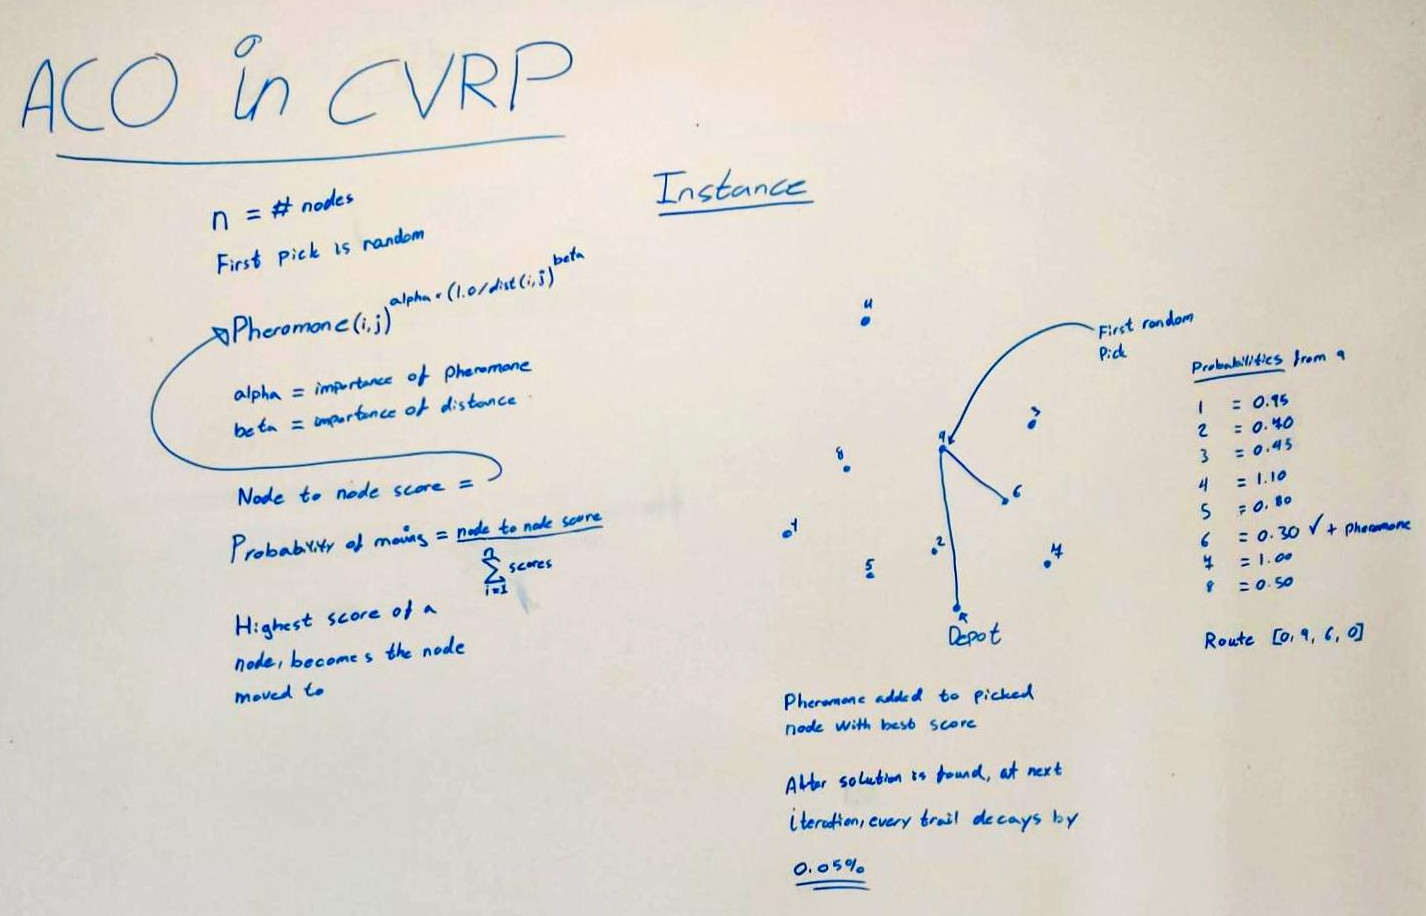
\includegraphics[width=0.9\textwidth]{ACO_Whiteboard.jpg}
	\label{fig:acowhiteboard}

\end{figure}

The complexity of the algorithm is $O(n)$ after initializing the pheromone matrix, due to the amount of checks from the current point 
it has to perform, which is \textit{n}\\

The psuedocode of the algorithm can be found in the appendices.

\section{Discussion}
Metaheuristics takes longer to execute, since they are not stopping until certain criteria is fulfilled. This criteria can be hard to reach and therefore, 
the algorithm can be running forever. In our two metaheuristic algorithms, the stopping criteria is the timespan of the running process. When the algorithms have been 
running for the set time, the process\' is stopped. \\
Our Simulated Annealing algorithm does run for a long time, but finds good solutions

\section{\\ FIGURES}

\newpage

\bibliographystyle{plain}
\bibliography{references}

\begin{appendices}

    \section{Metaheuristic - Ant Colony Optimization - Pseudocode}
    \begin{algorithm}[!ht]
        \caption{Metaheuristic - Ant Colony Optimization}
        \begin{algorithmic}[1]
            \State $\var{global\_best\_route} \gets \text{empty route/array}$
            \Function{algorithm}{}
                \While{A maximum number of iterations or a time limit has passed}
                    \State $\var{local\_best\_route} \gets \text{empty route/array}$
                    \State $\var{current\_route} \gets \text{empty route/array}$
                    \State $\var{capacity} \gets 0$
                    \State $\var{alpha} \gets \text{A random number}$
                    \State $\var{beta} \gets \text{A random number greater than alpha}$
                    \State $\var{evaporation} \gets \text{Some small number}$
                    \State $\var{pheromone\_matrix} \gets \text{Contains every pheromone for each pair}$
                    \State $\var{sum\_of\_all\_pheromone} \gets \text{The summation of the pheromone\_matrix}$
                    
                    \For{${first\_point} \gets 0$ to \text{length of data}}
                        \For{${second\_point} \gets 0$ to \text{length of data}}
                            \If{${first\_point} \neq {second\_point}$}
                                \State $\var{pheromone\_matrix(first, second)} \gets 1 / distance}$
                                \State $\var{sum\_of\_all\_pheromone} \gets \text{append calculated pheromone to the sum}$
                            \EndIf
                        \EndFor
                    \EndFor
    
                    \State Pick a random point for the list of points. 
                    \State Mark it as visited
                    \State Append it to the routes
                    \State Keep storage of the previous score
    
                    \While{${point} \neq \text{visited in list}$}
                        \For{key in \text{pheromone\_matrix}}
                            \State Calculate and store the Score-equation
                            \State Calculate and store the Probability-equation
                            \If{the new score \lt previous score \&\& key is not visited}
                                \State Set the key of the request to the point moved to
    
                            \EndIf
                        \EndFor
    
                        \State Append Newpheromone-equation to the trail of the point moved to
    
                        \If{Capacity of picked point \leq Capacity Constraint}
    
                            \State Capacity capacity of request
                            \State Append picked point to \var{current\_route}
                            \State Mark picked point as visited
                            \State Set picked point to the current point
                            \State Set previous score to 0
    
                        \Else
                            \State Reset \var{current\_route} and append picked point to new route
                            \State Mark point as visited
                            \State{$\var{capacity} \gets 0$}
                            \State{$\var{capacity} \gets capacity of picked point$}
                            \State Set previous score to 0
                        \EndIf
                    \EndWhile
                    \If{\var{current\_route} is better than \var{local\_best\_route}}
                        \State $\var{local\_best\_route} \gets \var{current\_route}$    
                    \EndIf
    
                    \If{\var{local\_best\_route} is better than \var{global\_best\_route}}
                        \State $\var{global\_best\_route} \gets \var{local\_best\_route}$  
                    \EndIf
    
                    \State loop through \var{pheromone\_matrix} and evaporate every pheromone trail by a small percentage
                \EndWhile
            \EndFunction
        \end{algorithmic}
    \end{algorithm}

\end{appendices}
\end{document}